
\appendix
\renewcommand{\thefigure}{A.\arabic{figure}}

\setcounter{figure}{0}    

\chapter{Bijlage}
\vspace{-3cm}
\begin{figure}[H]
	\centering
	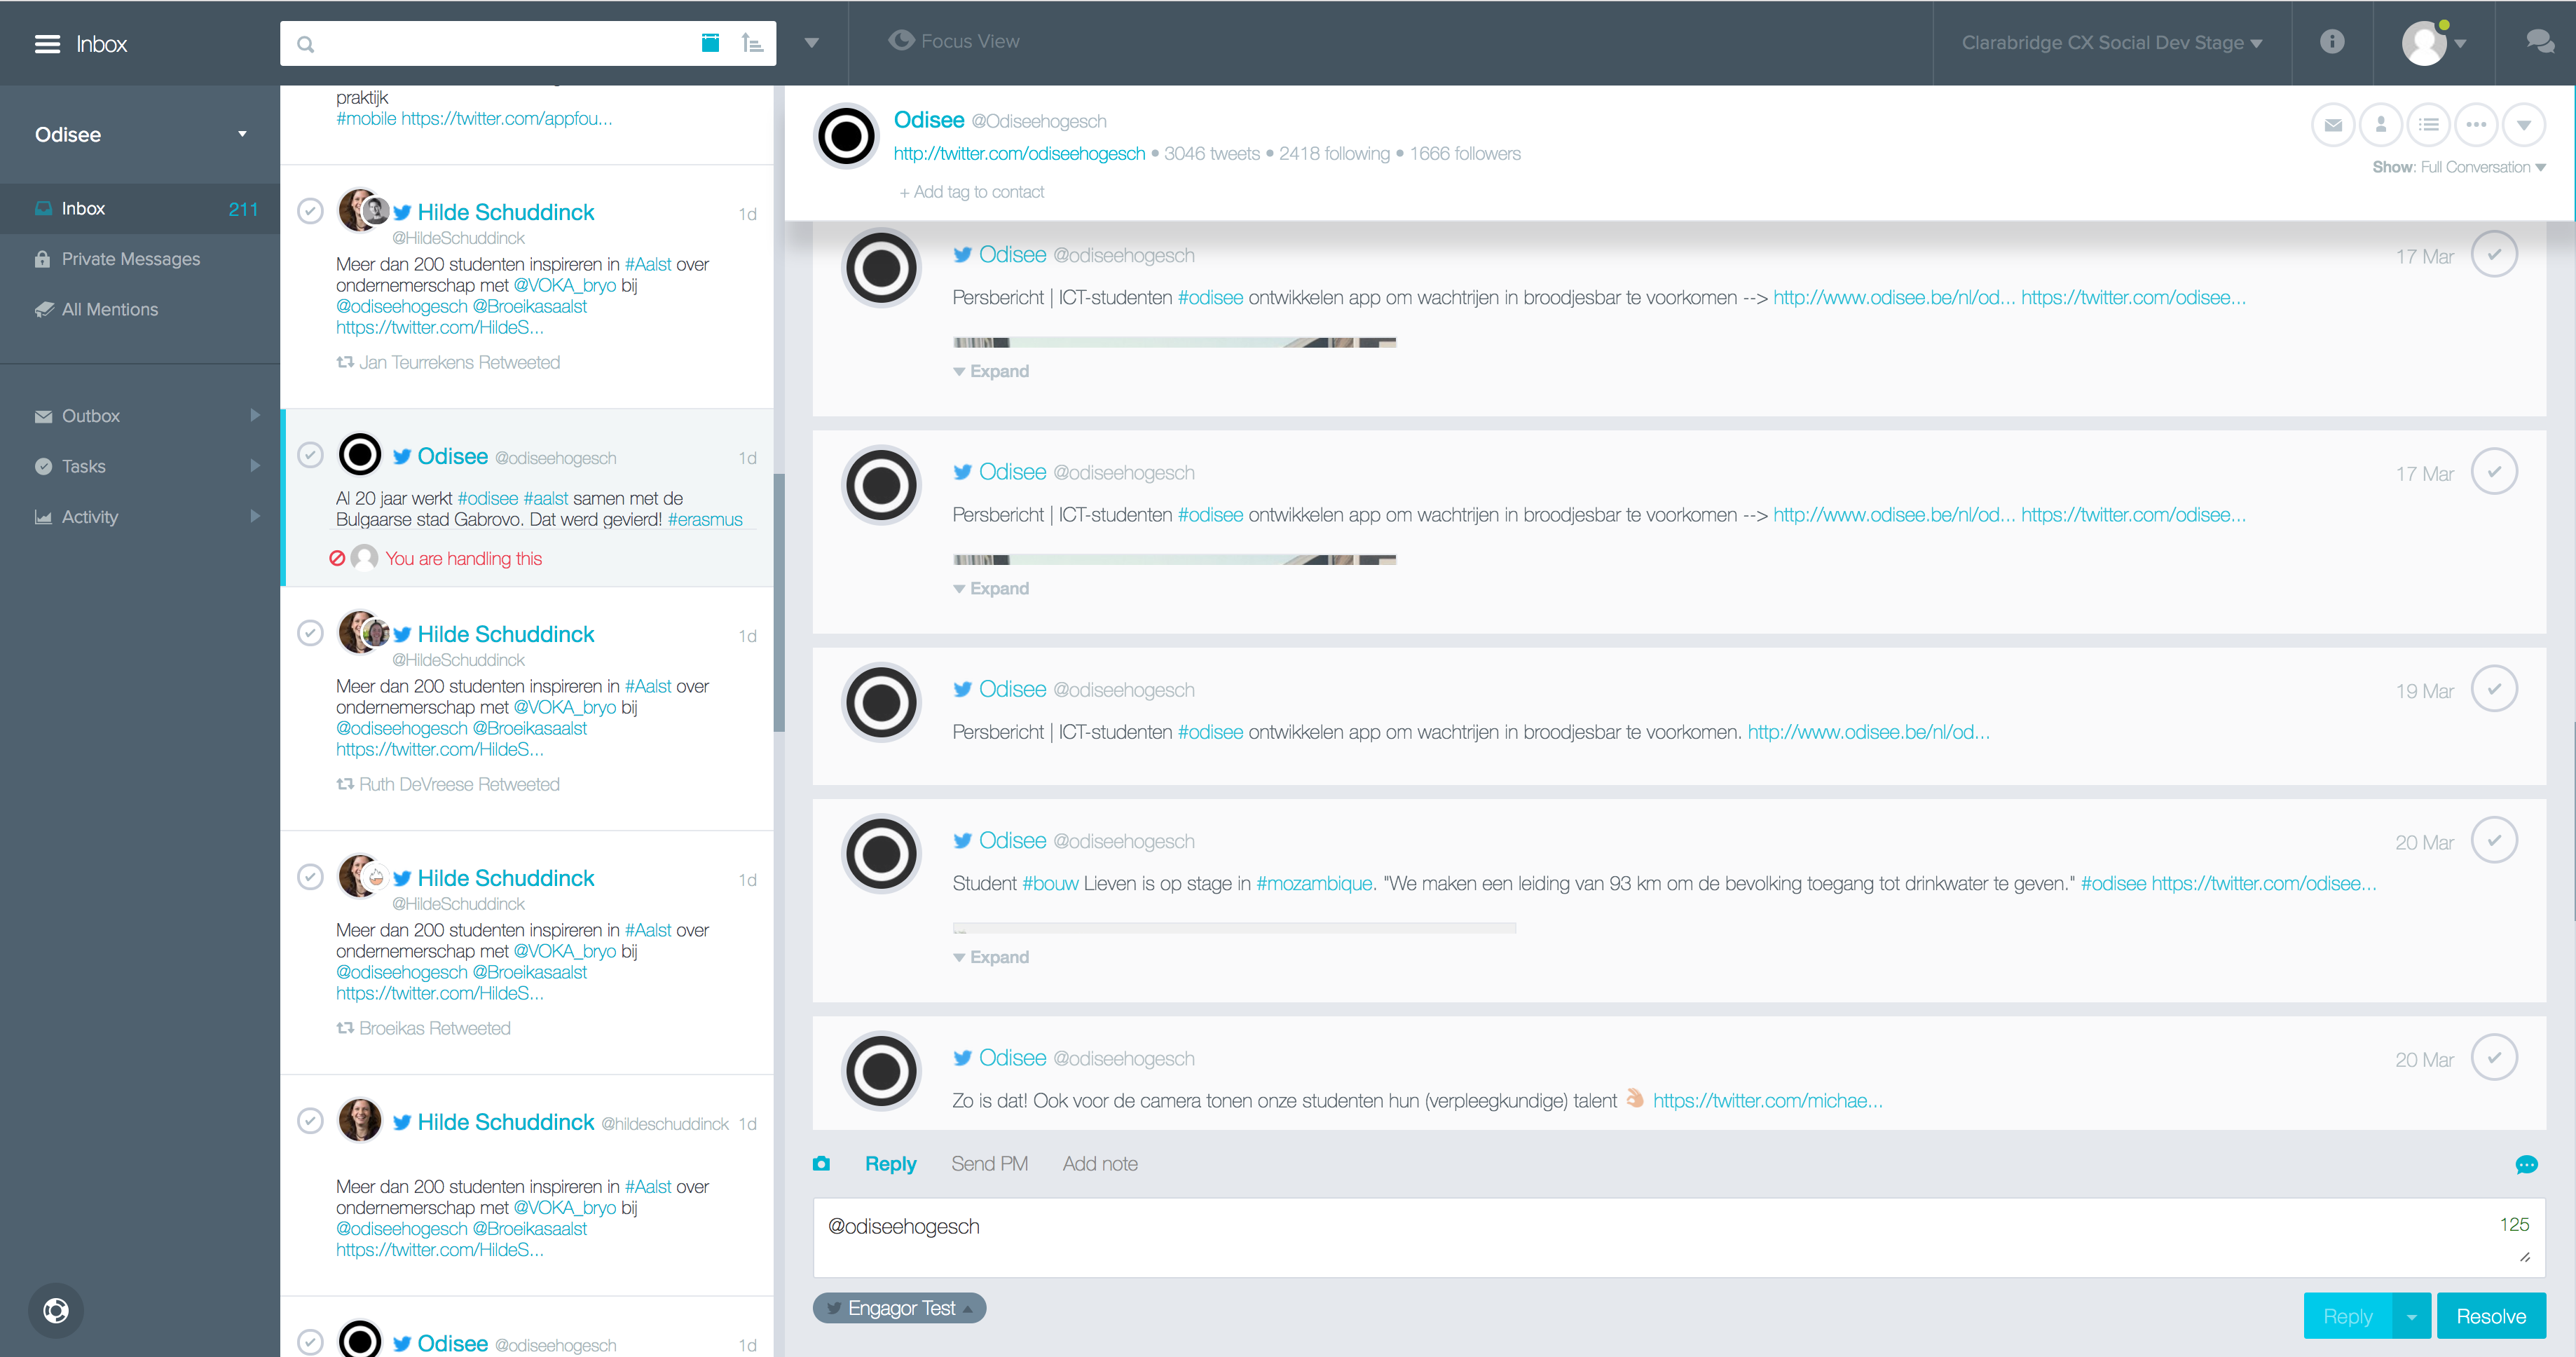
\includegraphics[width=1\textwidth]{Figuren/Inbox.png}
	\caption{Inbox CX Social \cite{EngagorScreenshots}} %\cite{Pouladzadeh}
	\label{fig:Inbox}
\end{figure} 

\begin{figure}[H]
	\centering
	
\includegraphics[width=1\textwidth]{Figuren/Performance.png}
	\caption{Performance CX Social \cite{EngagorScreenshots}} %\cite{Pouladzadeh}
	\label{fig:Performance}
\end{figure} 


\begin{figure}[H]
	\centering
	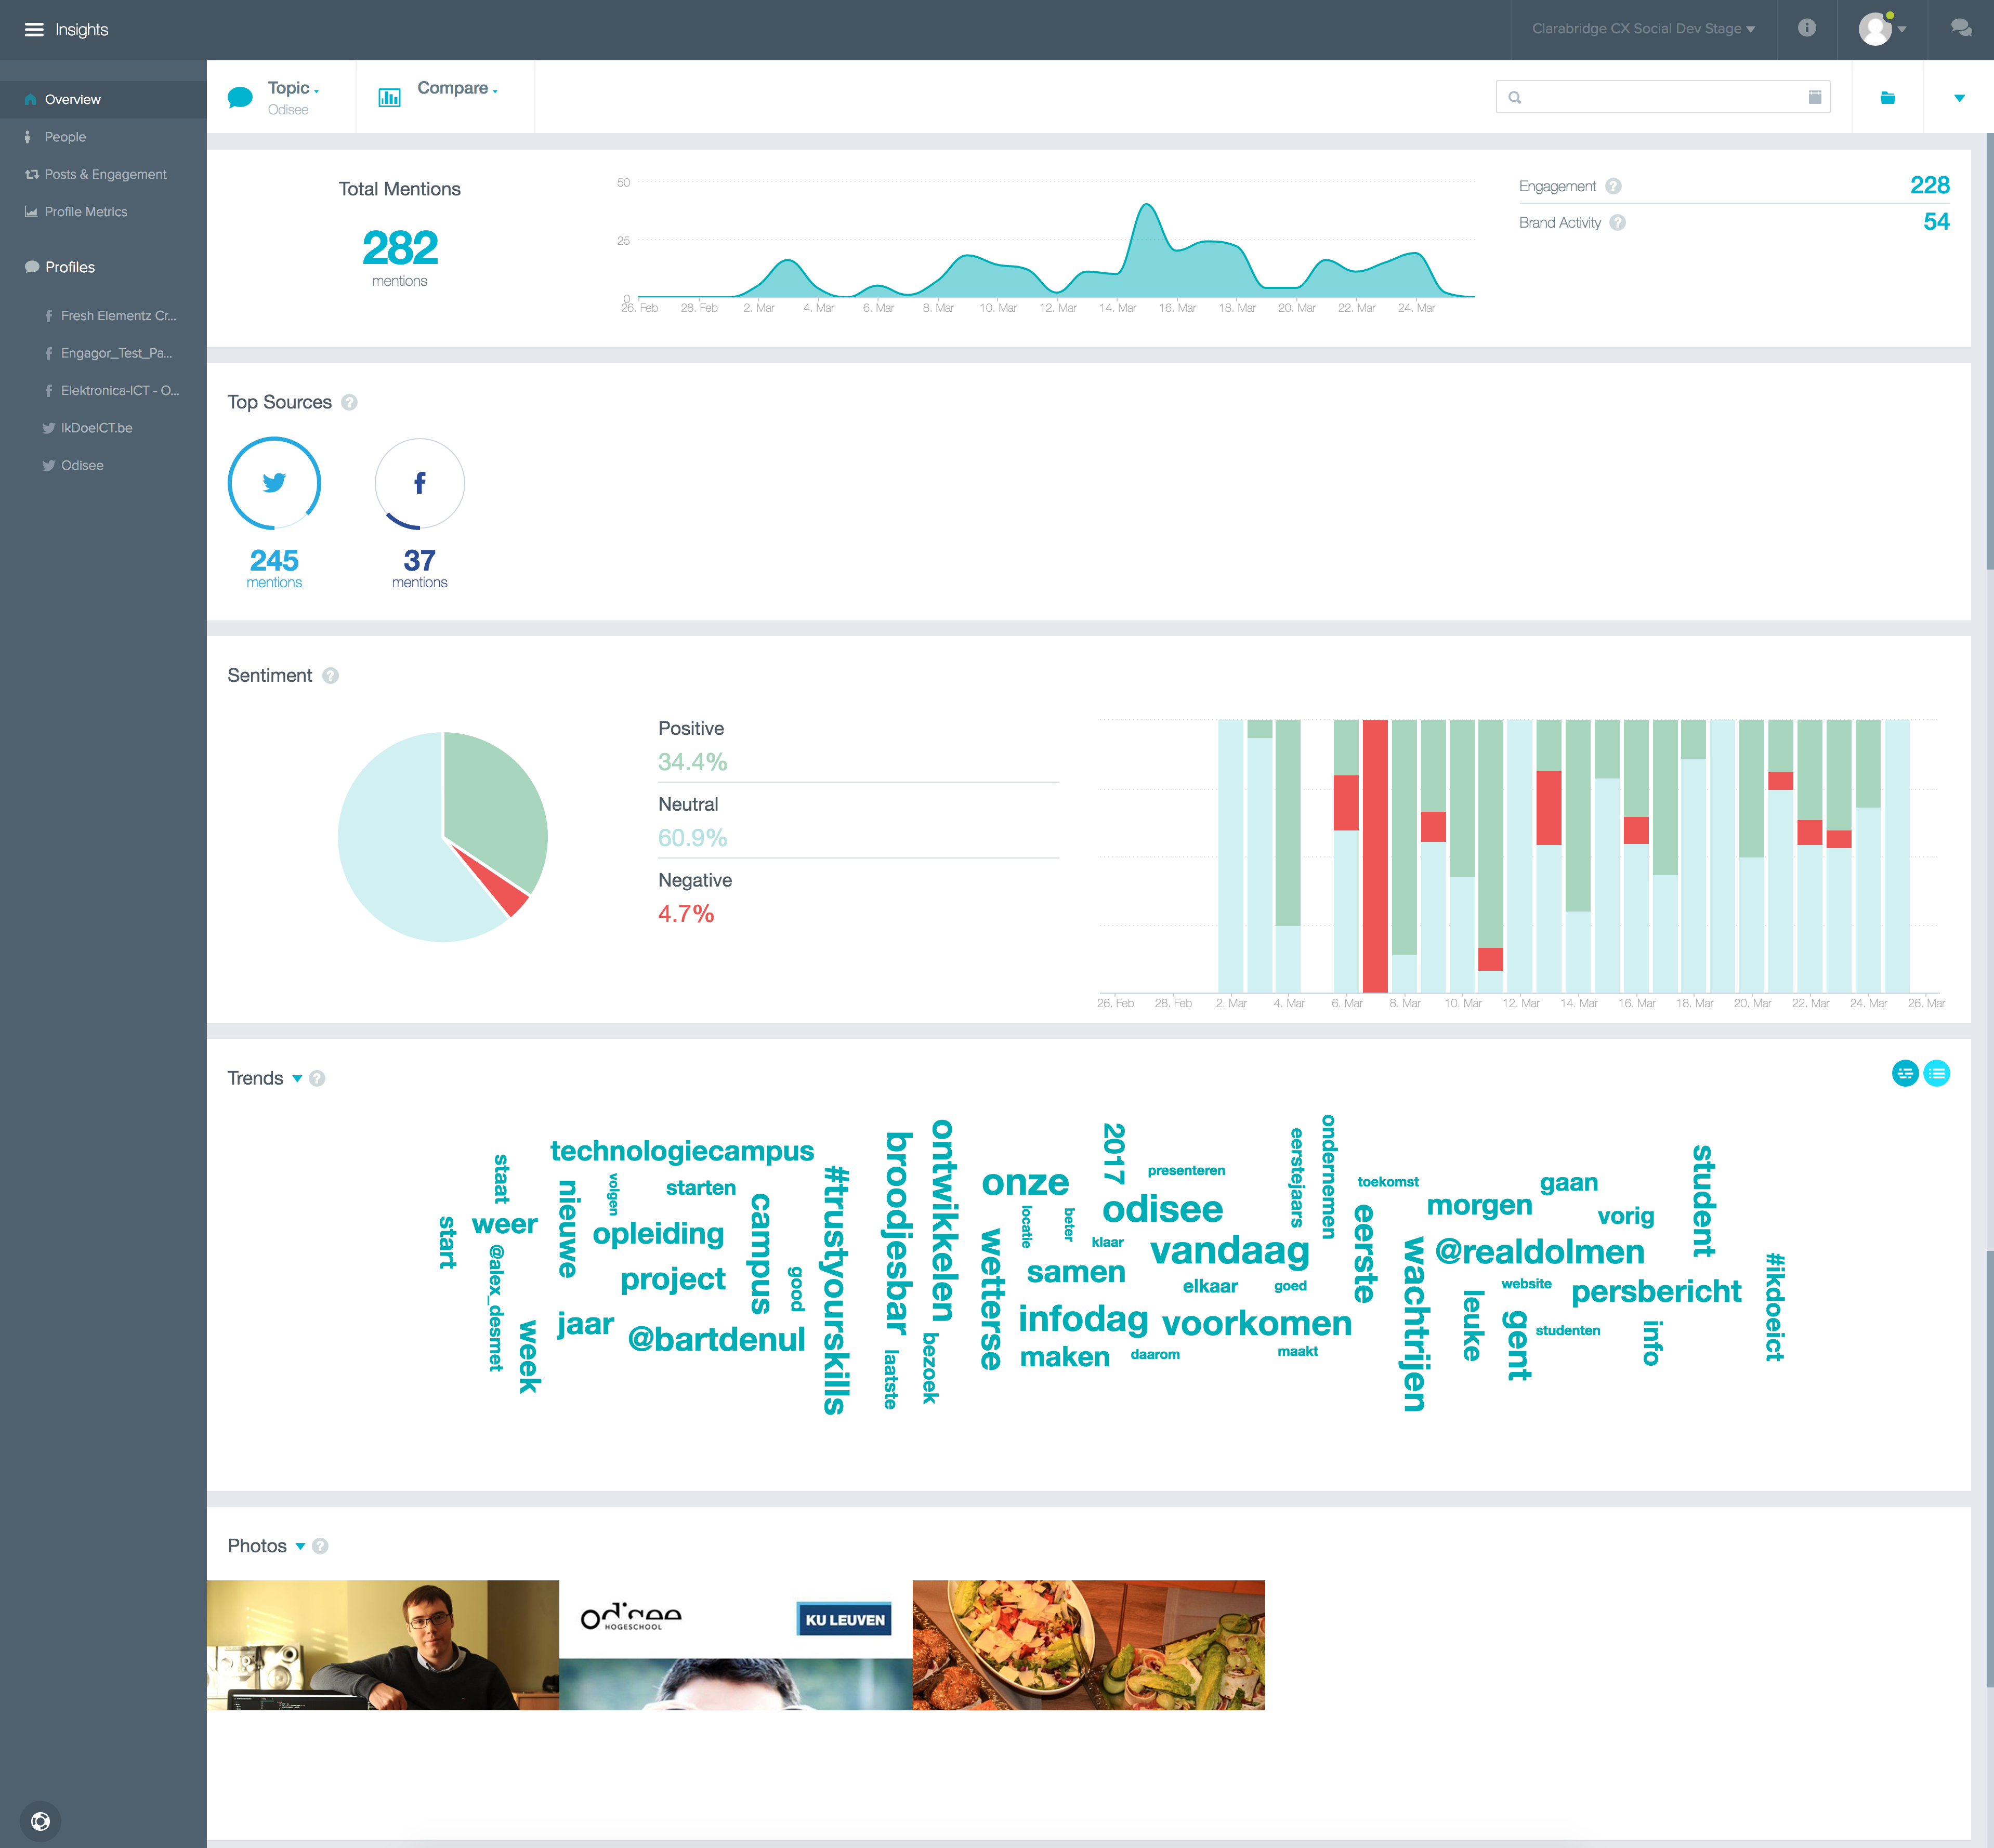
\includegraphics[width=1\textwidth]{Figuren/Insights.png}
	\caption{Insights CX Social \cite{EngagorScreenshots}} %\cite{Pouladzadeh}
	\label{fig:Insights}
\end{figure} 








\iffalse
\section{Theme Component}
\begin{lstlisting}[language=javascript]
var Theme = React.createClass({
propTypes: {
action: React.PropTypes.string.isRequired,
accountId: React.PropTypes.string.isRequired,
colors: React.PropTypes.array,
csrfToken: React.PropTypes.string.isRequired,
theme: React.PropTypes.object,
services: React.PropTypes.array.isRequired,
initialCoverImage: React.PropTypes.array,
initialAvatarImage: React.PropTypes.array,
selectedColor: React.PropTypes.string,
annotations: React.PropTypes.string,
showButton: React.PropTypes.bool,
isAllowedAnnotationsUpdate: React.PropTypes.bool.isRequired
},
getInitialState: function () {
return {
saving: false,
}
},
getActiveColor: function () {
return (
this.state.selectedColor || this.props.selectedColor
).slice(0);
},
getDefaultProps: function () {
return {
themeSets: []
};
},
getAnnotations: function () {
return (
this.state.annotations || this.props.annotations
);
},
componentDidUpdate: function () {
//window.secretProfileManagerAnnotations = this.getAnnotations();

},
componentWillUnmount: function () {
$(ThemeDispatcher).off('annotations', this.annotationHandler);
$(ThemeDispatcher).off('request-annotations', this.handleAnnotations);

//delete window.secretProfileManagerAnnotations;
},
getThemeName: function () {
return (
(this.refs.name) ? this.refs.name.value : '' || this.state.name || this.props.theme.name
).slice(0);
},
capitalize: function (string) {
return string.substring(0, 1).toUpperCase() + string.slice(1);
},
onSubmit: function () {
if (this.shouldDisableSubmit()) {
event.preventDefault();
}

this.setState({saving: true});
},
annotationHandler: function (event, annotations) {
this.setState({annotations: annotations});
},
componentWillMount: function () {
//window.secretProfileManagerAnnotations = this.getAnnotations();
},
handleAnnotations: function () {
$(ThemeDispatcher).trigger('response-annotations', this.getAnnotations());
},
componentDidMount: function () {
$(ThemeDispatcher).on('annotations', this.annotationHandler);
$(ThemeDispatcher).on('request-annotations', this.handleAnnotations);

},
shouldDisableSubmit: function () {
return (
(!this.refs.name || (this.refs.name && this.refs.name.value.trim() === '')) ||
(!this.refs.service || (this.refs.service && this.refs.service.value === ''))
//|| !this.state.imagesChanged
);
},
onImageChange: function () {
this.setState({imagesChanged: true});
},
getService: function () {
return (
this.state.service || this.props.theme.service
).slice(0);
},
renderError: function (error) {
return (
<p className="color-error">{error}</p>
);
},
renderTheme: function () {
var profileDesign = this.renderProfileDesign();


var deleteButton = null;
if (this.props.theme.id) {
var action = '/account/' + this.props.accountId + '/profile-manager/' + this.props.theme.id + '/delete';
deleteButton = (
<a href={action} className="button danger">
Delete
</a>
);
}

return (
<form className="profile-form" action={this.props.action} method="POST" onSubmit={this.onSubmit}>
<CsrfInput token={this.props.csrfToken}/>
<section className="profile-general fieldset-enclosed">
<h4 className="fieldset-title">General</h4>
<div className="default-row">
<div className="default-label">
<label htmlFor="themeName">
Name
</label>
</div>
<div className="default-field">
<input type="text" id="themeName" name="name" value={this.getThemeName()}
className={this.state.saving && this.getThemeName() === '' ? 'error fieldset-input' : 'fieldset-input'}
ref="name" onChange={function (event) {
this.setState({name: event.target.value});
}.bind(this)}/>
</div>
</div>
<div className="default-row">
<div className="default-label">
<label htmlFor="service">
Service
</label>
</div>
<div className="default-field">
<select
className={this.state.saving && this.state.service === '' ? 'error fieldset-input' : 'fieldset-input'}
id="service" name="service" ref="service" value={this.getService()}
onChange={function (event) {
this.props.theme.service = event.target.value;
this.setState({service: event.target.value});
}.bind(this)}>
{this.props.services.map(function (service) {
return <option key={service} value={service}>{this.capitalize(service)}</option>
}.bind(this))}
</select>
</div>
</div>
</section>
<section className="profile-design fieldset-enclosed left">
<h4 className="fieldset-title">Design</h4>
<div className="profile-design-preview">
{profileDesign}
</div>
<input type="hidden" name="annotations" value={this.getAnnotations()}/>
<div className="profile-actions right">
<button type="submit" name="submit" className="primary" value="Save"
disabled={this.shouldDisableSubmit() || this.state.saving}>
Save
</button>
<a href={'/account/' + this.props.accountId + '/profile-manager'} className="button">
Cancel
</a>
{deleteButton}
</div>
</section>
</form>
)
},
renderProfileDesign: function () {
var profileDesign = null;
var service = this.getService();

if (service == 'facebook') {
profileDesign = (
<div className="profile-design-page facebook-design left">
<ProfileManagerImageUploader initialImages={this.props.initialCoverImage} type="cover"
service={this.getService()}
onImageChange={this.onImageChange}
isAllowedAnnotationsUpdate={this.props.isAllowedAnnotationsUpdate}></ProfileManagerImageUploader>
<div className="profile-first-col left">
<ProfileManagerImageUploader initialImages={this.props.initialAvatarImage} type="avatar"
service={this.getService()}
onImageChange={this.onImageChange}></ProfileManagerImageUploader>
<div className="fake-title left-col-text-placeholder left-col-titles-placeholder"></div>
<div className="fake-sub-title-large sub-title-placeholder left-col-titles-placeholder"></div>

<div
className="fake-sub-title-large sub-title-placeholder left-col-titles-placeholder second-paragraph"></div>
<div className="fake-sub-title-small sub-title-placeholder left-col-titles-placeholder"></div>
<div className="fake-sub-title-large sub-title-placeholder left-col-titles-placeholder"></div>
</div>
<div className="profile-second-col left">
<div className="profile-sub-cover-placeholder"></div>
<div>
<div className="profile-sub-cover-left left">
<div className="profile-left-box-placeholder"></div>
<div className="profile-left-box-placeholder"></div>
</div>
<div className="profile-sub-cover-right right">
<div className="profile-right-box-placeholder"></div>
<div className="profile-right-box-placeholder"></div>
<div className="profile-right-box-placeholder"></div>
</div>
</div>
</div>
</div>
);
}
else {
profileDesign = (
<div>
<ProfileManagerImageUploader initialImages={this.props.initialCoverImage} type="cover"
service={this.getService()}
onImageChange={this.onImageChange}
isAllowedAnnotationsUpdate={this.props.isAllowedAnnotationsUpdate}></ProfileManagerImageUploader>
<div className="profile-design-page left">
<ProfileManagerImageUploader initialImages={this.props.initialAvatarImage} type="avatar"
service={this.getService()}
onImageChange={this.onImageChange}></ProfileManagerImageUploader>
<div className="profile-first-col left">
<div className="fake-title left-col-text-placeholder left-col-titles-placeholder"></div>
<div
className="fake-sub-title-large sub-title-placeholder left-col-titles-placeholder"></div>

<div
className="fake-sub-title-large sub-title-placeholder left-col-titles-placeholder second-paragraph"></div>
<div
className="fake-sub-title-small sub-title-placeholder left-col-titles-placeholder"></div>
<div
className="fake-sub-title-large sub-title-placeholder left-col-titles-placeholder"></div>
<div className="link-button-container">
<div className="link-color">
<ColorPicker selectedColor={this.props.selectedColor}
showButton={this.props.showButton}
colors={this.props.colors} buttonText='Link Color'
onChange={function (color) {
this.setState({selectedColor: color});
}.bind(this)}></ColorPicker>
</div>
</div>
</div>
<div className="profile-second-col left">
<div className="avatar-feed left"></div>
<div className="post-feed left">
<div className="post-feed-title-placeholder text-placeholder"></div>
<div className="post-feed-image-placeholder"></div>
<div className="post-feed-title-placeholder text-placeholder second-post"></div>
<div className="post-feed-text-placeholder-large text-placeholder"></div>
<div className="post-feed-text-placeholder-medium text-placeholder"></div>
<div className="post-feed-text-placeholder-large text-placeholder"></div>
<div className="post-feed-text-placeholder-small text-placeholder"></div>
</div>
</div>
<div className="profile-third-col left"></div>
</div>
</div>
);
}

return (
<div>
{profileDesign}
</div>
);
},
render: function () {
return (
<div>
{this.renderTheme()}
</div>
);
}
});
\end{lstlisting}




\begin{lstlisting}[language=javascript]
handleAnnotations: function (event, data) {
if (data) {
this.canvas.loadFromJSON(data, function () {
if (this.props.service === 'twitter') {
this.renderLimitationBars(40);
}

this.canvas.getObjects().forEach(function (object) {
if (object.type === 'image') {
object.remove();
}
});

fabric.Image.fromURL(this.getSource(this.props.image), function (image) {
image.center();
image.scaleToWidth(this.refs.container.offsetWidth);
image.setCoords();
this.canvas.add(image);
this.canvas.sendToBack(image);
}.bind(this));

this.canvas.renderAll();

this.setState({rendering: false, annotations: data});
}.bind(this));
}
else {
fabric.Image.fromURL(this.getSource(this.props.image), function (image) {
image.center();
image.scaleToWidth(this.refs.container.offsetWidth);
image.setCoords();
this.canvas.add(image);
this.canvas.sendToBack(image);
}.bind(this));
}
}
\end{lstlisting}

/// PUT IN BIJLAGE
\begin{lstlisting}[language=javascript]
componentDidMount: function () {
this.canvas.on({'object:selected': function () {
var object = null;
if (this.isTextSelected()) {
object = this.canvas.getActiveObject();

var kpiType = '';
if (object.textType === 'kpi') {
kpiType = object.kpiType;
object.set({'borderColor': '#f68d2e', 'cornerColor': '#f68d2e'});
} else if (object.textType === 'textbox') {
object.set({'borderColor': '#00b4d0', 'cornerColor': '#00b4d0'});
}

this.setState({
currentSettings: {
fontSize: object.getFontSize(),
fontWeight: object.getFontWeight(),
fontFamily: object.getFontFamily(),
fontStyle: object.getFontStyle(),
fontColor: object.getFill(),
textAlign: object.getTextAlign(),
}, textSelected: true, objectInfo: kpiType
});
}
else {
this.setState({
currentSettings: {
fontSize: '',
fontWeight: '',
fontFamily: '',
fontStyle: '',
fontColor: '#FFF',
textAlign: '',
}, textSelected: false
});
}
}.bind(this)});
}
\end{lstlisting}


\fi